\documentclass[11pt]{beamer}
\usetheme{Madrid}
\usepackage[utf8]{inputenc}
\usepackage[english,serbian]{babel}
\usepackage{amsmath}
\usepackage{amsfonts}
\usepackage{amssymb}
\usepackage{graphicx}
\DeclareMathOperator {\argmin}{argmin}

\author{Nemanja Protić, Kristijan Petronijević, Nera Zejak, Eleonora Jovanović Kisseleva}
\title{Pametni (električni) automobili u 2022. godini}
% Informe o seu email de contato no comando a seguir
% Por exemplo, alcebiades.col@ufes.br
%\setbeamercovered{transparent} 
\setbeamertemplate{navigation symbols}{} 

\institute[]{Matematički fakultet Univertziteta u Beogradu} 
\date{08. decembar 2022.} 
%\subject{}

% ---------------------------------------------------------
% Selecione um estilo de referência
\bibliographystyle{apalike}

%\bibliographystyle{abbrv}
%\setbeamertemplate{bibliography item}{\insertbiblabel}
% ---------------------------------------------------------

% ---------------------------------------------------------
% Incluir os slides nos quais as referências foram citadas
%\usepackage[brazilian,hyperpageref]{backref}

%\renewcommand{\backrefpagesname}{Citado na(s) página(s):~}
%\renewcommand{\backref}{}
%\renewcommand*{\backrefalt}[4]{
%	\ifcase #1 %
%		Nenhuma citação no texto.%
%	\or
%		Citado na página #2.%
%	\else
%		Citado #1 vezes nas páginas #2.%
%	\fi}%
% ---------------------------------------------------------

\begin{document}

\begin{frame}
\titlepage
\end{frame}

\begin{frame}{Literatura}
\begin{itemize}

\item \textcolor{black}{{\footnotesize Policy advice:}} {\footnotesize \url{ https://policyadvice.net/insurance/insights/electric-car-statistics}}
\item \textcolor{black}{{\footnotesize Wikipedia:}} {\footnotesize \url{ https://en.wikipedia.org/wiki/Electric_car#History}}
\item \textcolor{black}{{\footnotesize Idaho National Laborator:}} {\footnotesize \url{  https://avt.inl.gov/sites/default/files/pdf/fsev/HistoryOfElectricCars.pdf}}
\item \textcolor{black}{{\footnotesize U.S Department of energy:}} {\footnotesize \url{  https://www.energy.gov/articles/history-electric-car}}
\item \textcolor{black}{{\footnotesize U.S. Department of energy:}} {\footnotesize \url{ttps://afdc.energy.gov/vehicles/how-do-all-electric-cars-work }}
\item \textcolor{black}{{\footnotesize Autorent:}} {\footnotesize \url{ https://autorentdoo.com/blog/modeli-automobila-koji-ce-obeleziti-2022-godinu-84.html./}}
\item \textcolor{black}{{\footnotesize Aljazeera:}} {\footnotesize \url{ https://balkans.aljazeera.net/news/technology/2022/10/27/u-prodaji-prvi-ruski-elektricni-automobil}}
\item \textcolor{black}{{\footnotesize UN Enviorment Programme:}} {\footnotesize \url{ https://www.unep.org/ietc/resources/report/future-electric-vehicles-and-material-resources-foresight-brief}}
\item \textcolor{black}{{\footnotesize City of Moreno Valley:}} {\footnotesize \url{ http://www.moval.org/mvu/ev-advantages.html}}
\end{itemize}
\end{frame}

\begin{frame}{Sadržaj}
\tableofcontents 
\end{frame}

\section{Uvod}

\begin{frame}{Uvod}
\begin{itemize}
    \item  Električni automobil  je automobil kojeg pokreće jedan ili više elektromotora, koristeći \textbf{električnu energiju} iz baterija, ili iz drugih izvora za skaldištenje električne energije.
\end{itemize}
\begin{table}[htb]
        \caption{Procenat kupljenih automobila sa električnim pogonom za 2022. godinu.}
        \label{tab:modelo_tabela}
        \centering
       \begin{tabular}{|c|c|c|c|} \hline
Država& Norveška& Island& Švedska\\ \hline
Procenat kupljenih pametnih automobila& 58\%& 18\%& 11\%\\ \hline
\end{tabular}
        
       
    \end{table}

\end{frame}

\section{Istorija}
\begin{frame}{Rana istorija}
\begin{itemize}
    \item Praktična električna vozila su se prvi put pojavila 90-ih godina 19. veka.
    \item Koristila su se kao privatna motorna vozila do 20. veka, kada je došlo do svetskog pada njihove upotrebe kao privatnih motornih vozila.
    \item Odlučujući momenat u ovom preokretu je bilo uvođenje \textbf{anlasera} 1912. godine. koji je zamenio druge metode pokretanja \textbf{SUS motora}.
    \item Na početku 21. veka interesovanje za njihovu upotrebu kao privatna vozila se ponovo povećalo.
\end{itemize}
\end{frame}

\begin{frame}{Moderni električni automobili}
\begin{itemize}
    \item Na početku 21. veka je došlo do porasta zabrinutosti zbog štete po životnu sredinu urzokovanu emisijama koje prave vozila koja rade na fosilnim gorivima.
    \item Zaslugu za povećanje interesovanja za električne automobile je bilo prouzrokovano od strane \textbf{dva događaja}.
    \item \textbf{Prvi događaj} je bio pojava \textbf{Toyota Prius-a} koji je postao prvo svetsko hibridno električno vozilo koje je imalo masivnu proizvodnju i postalo najprodavaniji hibrid širom sveta u poslednjoj deceniji.
    \item \textbf{Drugi događaj} je bila vest u 2006. godini o tome da će kompanija Tesla Motors početi da proizvodi model luksuznih električnih sportskih automobila, nazvan \textbf{Tesla Rodste}r, koji je postao prvi potpuno električni automobil legalan na putu koji putuje više od 320 km sa jednim punjenjem.
\end{itemize}
\end{frame}

\section{Princip rada}
\begin{frame}{Princip rada elektricnih automobila}
\begin{itemize}
\item Električni automobili rade zahvaljujući energiji koju crpe iz punjivih baterija.
\item Obavezan korak je konverzija jednosmerne električne energije u naizmeničnu.
\item \textbf{Potenciometri} - promenljiv otpor koji odoleva struji u strujnom kolu.
\item \textbf{Regulator} - uređaj koji kontroliše količinu električne energije koja se doprema motoru.
\item Konverzija energije je ključni korak koji omogućava pokretanje motora, okretanje točkova i kretanje automobila.
\end{itemize}
\end{frame}

\section{Modeli automobila}

\begin{frame}{Modeli automobila koji su obeležili 2022. godinu}{\thesection \, \secname}

\begin{itemize}
\item Automobilska industrija je zabeležila ogroman pad u periodu izmedju 2020 - 2021. godine.
\item Zaustavljen proizvodni proces dao je prostor za rad na novim idejama koje su kasnije implementirane u nove modele.
\item Evropska komisija je uvela obavezu svim proizvođačima za ugradnju uređaja za "inteligentno podešavanje brzine".
\end{itemize}
\end{frame}

\begin{frame}{Modeli automobila koji su obeležili 2022. godinu}
Neki od modela koje su predstavile poznate auto kuće su:
\begin{itemize}
\item Škoda Enyaq iV
\item Renault Austral
\item Mercedes-Benz Vision EQXX
\item Evolute i-Pro
\item Drako Dragon

\begin{figure}[h]
        \centering
        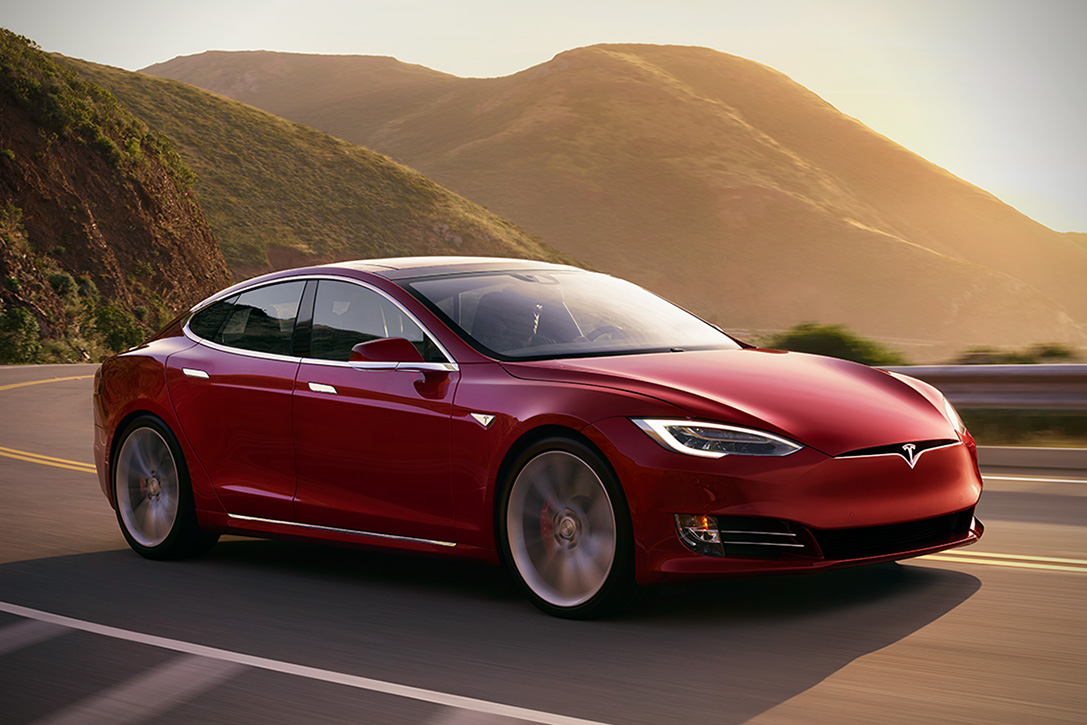
\includegraphics[width=60mm, scale=0.5]{tesla.jpeg}
        \label{fig:tesla.jpeg}
        \end{figure}

\end{itemize}

\end{frame}

\section{Zaključak}

\begin{frame}{Zaključak}
\begin{itemize}
\item Električni automobili su unapredili saobraćaj time što su smanjili emisije štetnih gasova i uveli veću sigurnost.
\item Potrošači na njih gledaju kao na investiciju, ali statistika kaže da su na dugoročnom planu isplativiji od regularnih automobila.
\item Zahtevniji su za održavanje od običnih vozila zbog kompleksnosti njihove strukture i često ne podležu osiguranju.
\end{itemize}

\end{frame}


\end{document}
